\chapter{\uppercase{Dataset}}\label{ch:datasets}  

  The collection of the dataset was one of the most laborious tasks in this project. There were criteria we were searching to find. These criteria are as follows,
  \begin{itemize}
    
  \item \textbf{Datasets availability:} There are old Arabic references which have a lot of Poems but not all these books were not available in a PDF or a Web pages format, and it was hard to find it.
    
  \item \textbf{The Poem with diacritics:} There are resources which have Arabic Poems, but it is much harder to find same with diacritics.
    
  \item \textbf{The amount of the dataset:} To have a successful project with good results we need a massive amount of data. From the previous work, We did not find this amount of data. The maximum number found was 1.5k. However, We were searching for around 1.5M record of classified Poems.

  
\item \textbf{Cleansing of this data:} There was a limitation for the datasets which we can consider it, or we can scrap it due to the limitation for the APIs or the ready datasets in this context.
  
\end{itemize}
To meet the above criteria and overcome it, We applied following,

\begin{itemize}

  \item \textbf{Datasets availability:} We have scrapped the Arabic datasets from two big poetry websites: \textarabic{الديوان}~\cite{diwan}, \textarabic{الموسوعة الشعرية}~\cite{PoetryEncyclopedia2016}. Both merged into one large dataset, and we open sourced it online ~\cite{ArabicpoetryDS}.

  \item \textbf{The Poem with diacritics:} We tried to get the most verses with the available diacritics, but the diacritics states are not consistent, So, a verse can be fully diacritics, Semi diacritics or without diacritics.

\item \textbf{The amount of the dataset:} The total number of verses is 1,862,046 poetic verses; each verse labeled by its meter (class), the poet who wrote it, and the age which it was written. There are 22 meters, 3701 poets and 11 ages; and they are Pre Islamic, Islamic, Umayyad, Mamluk, Abbasid, Ayyubid, Ottoman, Andalusian, the era between Umayyad and Abbasid, Fatimid and modern. We are only interested in the 16 classic meters which attributed to Al-Farahidi, and they are the majority of the dataset with a total number of 1,722,321 verses. Figure~\ref{fig:data_size_distribution} shows the distribution of the verses per meter. %@@@ add datasets figures percentage per class
  
\item \textbf{Cleansing of this data:} Dataset was not cleaned enough for usage in this research, but we have applied cleansing rules explained in details in Data Preparation and Cleansing section~\ref{sec:data_clens}. We also open sourced all the code scripts used in our online repository~\cite{HCILAB_ArabicPoetry_2018}.
\end{itemize}

\begin{figure}
	\centering
	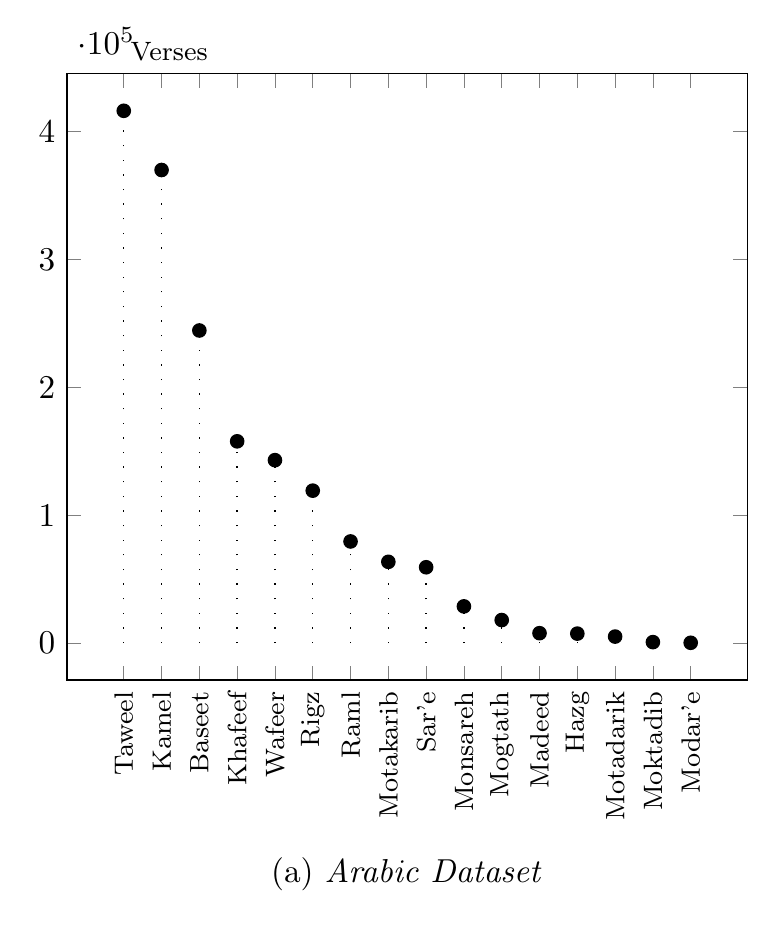
\begin{tikzpicture}[scale=1.2]
	\begin{axis}[
    symbolic x coords={Taweel,
   Kamel,
   Baseet,
   Khafeef,
   Wafeer,
   Rigz,
   Raml,
   Motakarib,
   Sar'e,
   Monsareh,
   Mogtath,
   Madeed,
   Hazg,
   Motadarik,
   Moktadib,
   Modar'e
    },
    xtick=data,
    % the following x label positioning does work here.
    every axis y label/.style= {at={( 0.15, 1.07)}, anchor=north},
    ylabel style={font=\footnotesize},
    xticklabel style = {font=\footnotesize},
    ylabel={Verses},
    height=8cm,
    x=0.4cm,
    x tick label style={rotate=90, anchor=east},
    enlarge y limits=0.07,
    name=left plot,%
    title=(a) \textit{Arabic Dataset},%
    title style={at={(0.5,-.4)}}%
  ]
    \addplot[ybar,color=black,mark=*, only marks,
	    point meta=explicit symbolic] coordinates {
        (Taweel, 416428)
        (Kamel,  370116)
        (Baseet, 244583)
        (Khafeef,     157880)
        (Wafeer,     143148)
        (Rigz,     119286)
        (Raml,     79560)
        (Motakarib,     63613)
        (Sar'e,     59370)
        (Monsareh,     28768)
        (Mogtath,     18062)
        (Madeed,     7808)
        (Hazg,     7468)
        (Motadarik,     5144)
        (Moktadib,     799 )
        (Modar'e,     288 )
    };

    \draw[loosely dotted] (axis cs:Taweel, 0) -- (axis cs:Taweel, 416428);
    \draw[loosely dotted] (axis cs:Kamel,  0) -- (axis cs:Kamel,  370116);
    \draw[loosely dotted] (axis cs:Baseet, 0) -- (axis cs:Baseet, 244583);
    \draw[loosely dotted] (axis cs:Khafeef,0) -- (axis cs:Khafeef,157880);
    \draw[loosely dotted] (axis cs:Wafeer, 0) -- (axis cs:Wafeer, 143148);
    \draw[loosely dotted] (axis cs:Rigz,   0) -- (axis cs:Rigz,   119286);
    \draw[loosely dotted] (axis cs:Raml,   0) -- (axis cs:Raml,   79560);
    \draw[loosely dotted] (axis cs:Motakarib, 0) -- (axis cs:Motakarib, 63613);
    \draw[loosely dotted] (axis cs:Sar'e, 0)   -- (axis cs:Sar'e, 59370);
    \draw[loosely dotted] (axis cs:Monsareh, 0) -- (axis cs:Monsareh,28768);
    \draw[loosely dotted] (axis cs:Mogtath, 0) -- (axis cs:Mogtath, 18062);
    \draw[loosely dotted] (axis cs:Madeed,  0) -- (axis cs:Madeed,  7808);
    \draw[loosely dotted] (axis cs:Hazg,    0) -- (axis cs:Hazg,    7468);
    \draw[loosely dotted] (axis cs:Motadarik,0) -- (axis cs:Motadarik, 5144);
    \draw[loosely dotted] (axis cs:Moktadib, 0) -- (axis cs:Moktadib,  799 );
    \draw[loosely dotted] (axis cs:Modar'e,  0) -- (axis cs:Modar'e,   288 );

\end{axis}



	\end{tikzpicture}%
	\caption{Arabic dataset Meter per class percentage ordered descendingly on x axis vs. corresponding meter name on y axis all class in the left of the red line (less than 1\% assume to be trimmed in some experiments).	}\label{fig:data_size_distribution}
\end{figure}

\section{Data Scraping}\label{sec:data_scrap}
To scrap the data from the website: \textarabic{الديوان}~\cite{diwan},ends up into such a problem just reduce your problem to the most smallest one. That means: First: Check if any "keywords" is set, if used. Then: Use your whole preamble and print the complete bibliography. If this ends up in the same error, your problem might be in your preamble. -> Reduction of preamble, until you get your bib printed. Adding slowly parts back to the preamble, until the error occurs again. That might show you, what lead to the warning.

 \textarabic{الموسوعة الشعرية}~\cite{PoetryEncyclopedia2016}, We used custom Python scripts for each websites to get the verses details. The script created with simple usage to pass the link we need to scrap. We will show two examples from both websites.
\begin{enumerate}
\item The First example, If we need to scrap a meter from \textarabic{الديوان} the website, for example Al-Tawil \\textit{https://www.aldiwan.net/poem.html?Word=\%C7\%E1\%D8\%E6\%ED\%E1\&Find=meaning}, We will pass this link to the script and the output file name. The script will start scraping and save the output in a CSV format. We can get the output similar than the output in table \ref{tables:Aldiwan_Sample}


% table: dal with diacritics
\begin{table}[H]
	\centering
	\begin{tabular}{c c c c c}
		%\hline
		\toprule
          \textbf{\small{\textarabic{البيت}}} & \small{\textbf{\textarabic{الشطر الأيسر}}} & \small{\textbf{\textarabic{الشطر الأيمن}}} &
\small{\textbf{\textarabic{البحر}}} & \small{\textbf{\textarabic{الشاعر}}} \\
		 %\hline
          \midrule
\makecell{\textarabic{رَجا شافع نسج المودّة بيننا}\\ \textarabic{ولا خيرَ في ودّ يكون بشافع}} &
\textarabic{ولا خيرَ في ودّ يكون بشافع} &                                                       \textarabic{رَجا شافع نسج المودّة بيننا} &                                                       \textarabic{الطويل}&
\textarabic{ابن نباته المصري}\\
          
		%\hline
		\bottomrule
	\end{tabular}
	\caption{Aldiwan scraping output example }\label{tables:Aldiwan_Sample}
\end{table}

\item Second Example, If we need to scrap the same meter from \textarabic{الموسوعة الشعرية} the website for example Al-Raml \textit{https://poetry.dctabudhabi.ae/\#/diwan/poem/126971}, We will pass this link to the script and the output file name. The script will start scraping and save the output in a CSV format. We can get the output similar than the output in table \ref{tables:ElMosoaa_Sample}


% table: dal with diacritics
\begin{table}[H]
	\centering
	\begin{tabular}{c c c c c c c c c}
		%\hline
          \toprule
\small{\textbf{\#}} &
\small{\textbf{\textarabic{البيت}}} &
\small{\textbf{\textarabic{الشطر الأيمن}}}&                        \small{\textbf{\textarabic{الشطر الأيسر}}} &
\small{\textbf{\textarabic{البحر}}}&                                 \small{\textbf{\textarabic{القافية}}}& \small{\textbf{\textarabic{الديوان}}}&                               \small{\textbf{\textarabic{الشاعر}}}&
\small{\textbf{\textarabic{العصر}}}\\
		 %\hline
          \midrule
1 &          
\makecell{\textarabic{من يرد مورد حب} \\ \textarabic{ظمأ بالشوق يزدد}} &
\textarabic{ظمأ بالشوق يزدد} &                                                        \textarabic{من يرد مورد حب} &                                                       \textarabic{الرمل}&
\textarabic{د}&
\makecell{\textarabic{الديوان} \\ \textarabic{الرئيسي}}&
\makecell{\textarabic{يعقوب الحاج}\\ \textarabic{ جعفر التبريزي}}&
\textarabic{الحديث}\\
          
		%\hline
		\bottomrule
	\end{tabular}
	\caption{Al-Mosoaa Elshearyaa scraping output example }\label{tables:ElMosoaa_Sample}
\end{table}
\end{enumerate}

We scrapped all the available datasets on both websites and merged them based on the common columns. Then we started the Data preparation tasks. We need to mention that, Not all diacritics was correctly available on all the websites. Also, We did not work to generate the diacritics for those datasets. So, we depended on whatever available without changing the data all the next sections is related to correction, preparation, and cleansing of the current datasets.
\newpage
\section{Data Preparation and Cleansing}\label{sec:data_clens}

Data preparation and cleansing tasks divided into multi-stages.
\begin{itemize}
\item Merge all scrapped datasets into one CSV file with a selection of the common columns in each file.
\item Remove the duplicates rows from the files in case we have any joined rows between both websites.
\item Filter the datasets on the 16 meters required as some data belonged to other non-famous or not original meters.
\item Remove many unnecessary white spaces which were useless.
\item Remove non-Arabic characters and the other web symbols.
\item Fix diacritics mistakes, such as the existence of two consecutive harakat, we have only kept one and have removed the other. %@@@add an example
\item Remove any \textit{harakah} comes after a white space, it removed as it is useless. %@@@add an example
\item We factored \textit{Shadaa}~\ref{def:shadaa_definition} to its original format explained in this example~\ref{tables:shadda_dal} previously.
\item We also factored \textit{Tanween}~\ref{def:tanween_definition} to its original format explained in this example~\ref{tables:Tanween_dal} previously.\footnote{\textit{We ignored the factorization of Alef-Mad  \textbf{\textarabic{ آ }} in our data preparation and transformation which can save more memory and shorten our encoding vectors}}
\end{itemize}

We need to highlight that the last two points are not a handcrafted feature. It is a factorization for the letter to its original format. This factorization will affect the size of the data in the memory and the letter representation in the vector. We will explain this part in details in the next chapter about encoding mechanism and the impact of the encoding type in the model training time and performance.







%%% Local Variables:
%%% mode: latex
%%% TeX-master: "../master"
%%% End:
